---
id: tkz-euclide-ejemplo-31
title: "Polígonos I"
description: "Dibuja dos polígonos y une vértices correspondientes con segmentos guía."
keywords: [poligono, segmento]
tags: [tkzDrawPolygon]
sort: 31
---
\documentclass[tikz,border=2mm]{standalone}
\usepackage{tkz-base}
\usepackage{tkz-euclide}

\begin{document}
    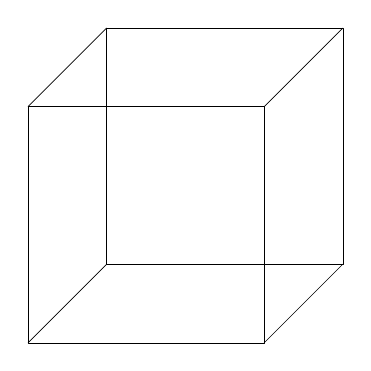
\begin{tikzpicture}
        % Define dos cuadriláteros A1B1C1D1 y A2B2C2D2.
        \tkzDefPoints{
            0/0/A1,
            3/0/B1,
            3/3/C1,
            0/3/D1,
            1/1/A2,
            4/1/B2,
            4/4/C2,
            1/4/D2%
        }
    
        % Dibuja ambos polígonos.
        \tkzDrawPolygon(A1,B1,C1,D1)
        \tkzDrawPolygon(A2,B2,C2,D2)
    
        % Conecta vértices correspondientes entre ambos polígonos.
        \tkzDrawSegment(A1,A2)
        \tkzDrawSegment(B1,B2)
        \tkzDrawSegment(C1,C2)
        \tkzDrawSegment(D1,D2)
    \end{tikzpicture}
\end{document}
